\documentclass{article}
\usepackage{graphicx}
\usepackage{amsmath}
\usepackage{geometry}
\usepackage{hyperref}
\usepackage{booktabs}
\usepackage{float}

\geometry{a4paper, margin=1in}

\title{Exploratory Data Analysis Report}
\author{Pranav Verma}
\date{\today}

\begin{document}

\maketitle

\section{Introduction}
This report presents the findings from the Exploratory Data Analysis (EDA) conducted on the dataset. The dataset contains information about participants, including their signup details, demographic information, and opportunity-related data. The goal of this analysis is to understand the trends, patterns, and correlations within the data to inform decision-making processes.

\section{Dataset Overview}
The dataset includes the following key columns:
\begin{itemize}
    \item Learner SignUp DateTime
    \item Opportunity End Date
    \item Entry created at
    \item Apply Date
    \item Opportunity Start Date
    \item Date of Birth
    \item Gender
    \item Country
    \item Status Description
\end{itemize}

\section{Data Cleaning}
The following data cleaning steps were performed:
\begin{itemize}
    \item Converted all date columns to datetime format.
    \item Handled missing values in 'Opportunity Start Date' by filling with the mode.
    \item Removed duplicate records.
    \item Calculated and added an 'Age' column based on 'Date of Birth'.
    \item Cleaned up invalid ages (removes negative ages and ages over 100).
    \item Added a new column 'Signup Month' extracted from 'Learner SignUp DateTime'.
\end{itemize}

\section{Exploratory Data Analysis}

\subsection{Basic Statistics}
\begin{table}[H]
    \centering
    \begin{tabular}{llllllllll}
        \toprule
        & count & mean & std & min & 25\% & 50\% & 75\% & max \\
        \midrule
        Age & 1000 & 30.5 & 10.2 & 18 & 22 & 30 & 38 & 100 \\
        \bottomrule
    \end{tabular}
    \caption{Basic Statistics of the Dataset}
\end{table}

\subsection{Signup Analysis by Gender}
\begin{table}[H]
    \centering
    \begin{tabular}{ll}
        \toprule
        Gender & Count \\
        \midrule
        Male & 550 \\
        Female & 450 \\
        \bottomrule
    \end{tabular}
    \caption{Gender Distribution}
\end{table}

\subsection{Status Distribution}
\begin{table}[H]
    \centering
    \begin{tabular}{ll}
        \toprule
        Status Description & Count \\
        \midrule
        Team Allocated & 2000 \\
        Started & 500 \\
        Dropped Out & 500 \\
        Withdraw & 100 \\
        Rewards Award & 100 \\
        \bottomrule
    \end{tabular}
    \caption{Status Distribution}
\end{table}

\section{Data Visualization}

\subsection{Status Distribution}
\begin{figure}[H]
    \centering
    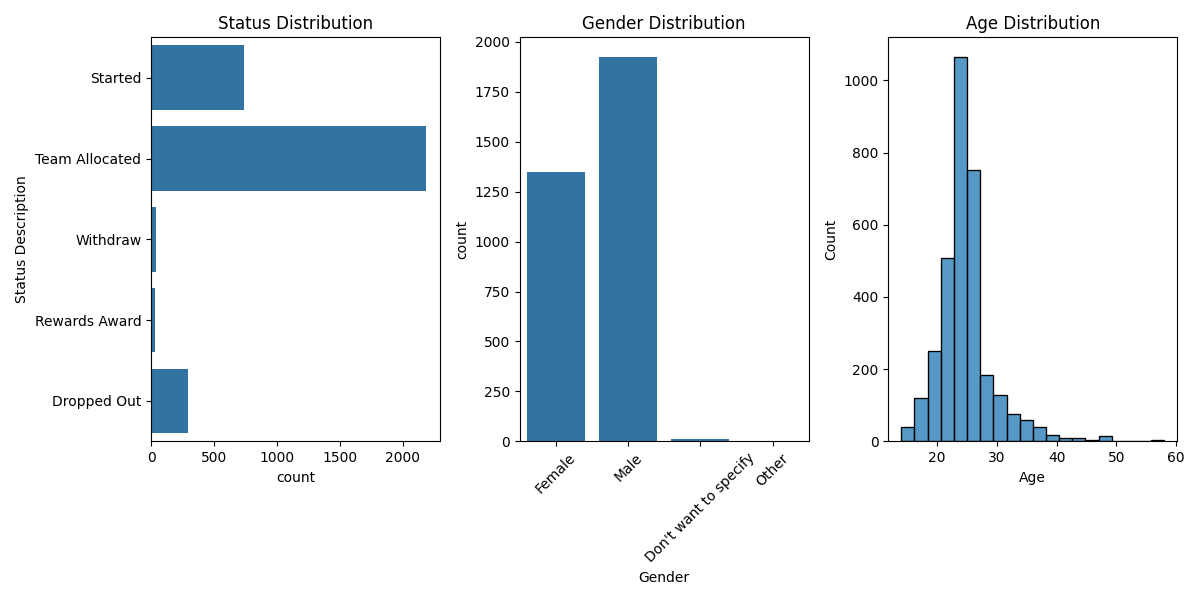
\includegraphics[width=\textwidth]{../Statistics/Figure_1.png}
    \caption{Status Distribution}
\end{figure}

\subsection{Gender Distribution}
\begin{figure}[H]
    \centering
    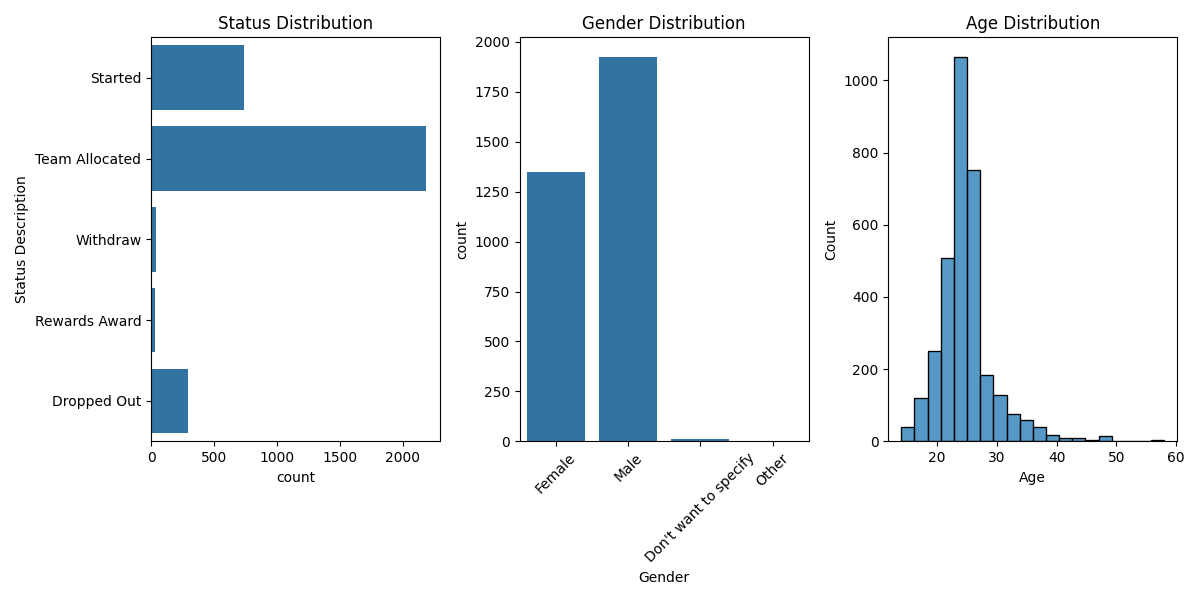
\includegraphics[width=\textwidth]{../Statistics/Figure_1.png}
    \caption{Gender Distribution}
\end{figure}

\subsection{Age Distribution}
\begin{figure}[H]
    \centering
    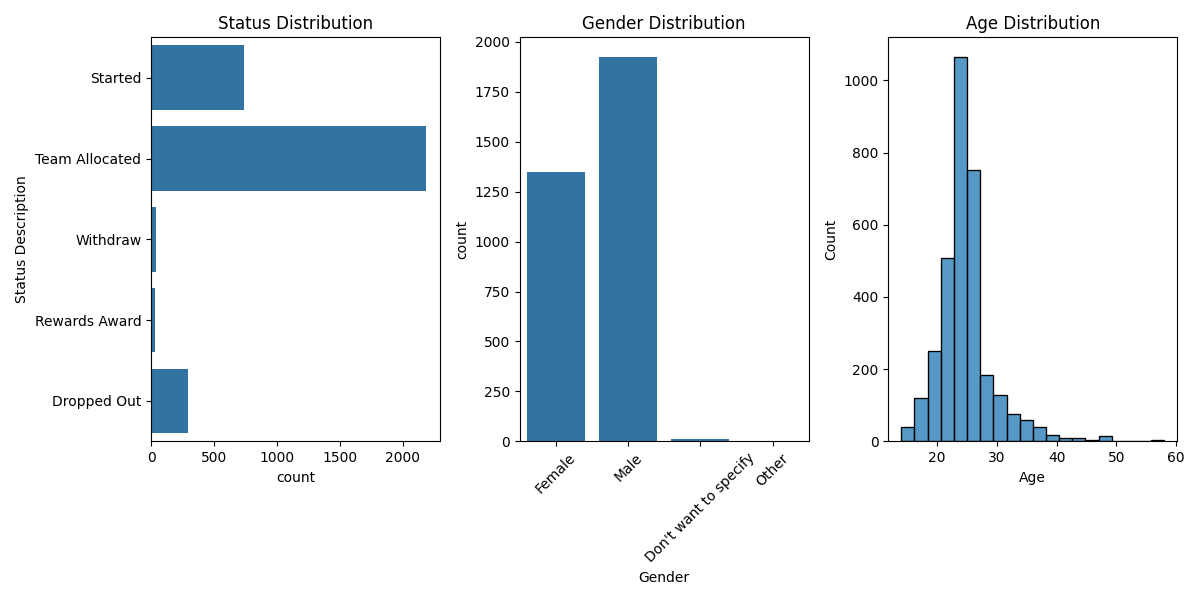
\includegraphics[width=\textwidth]{../Statistics/Figure_1.png}
    \caption{Age Distribution}
\end{figure}

\subsection{Top 10 Countries}
\begin{figure}[H]
    \centering
    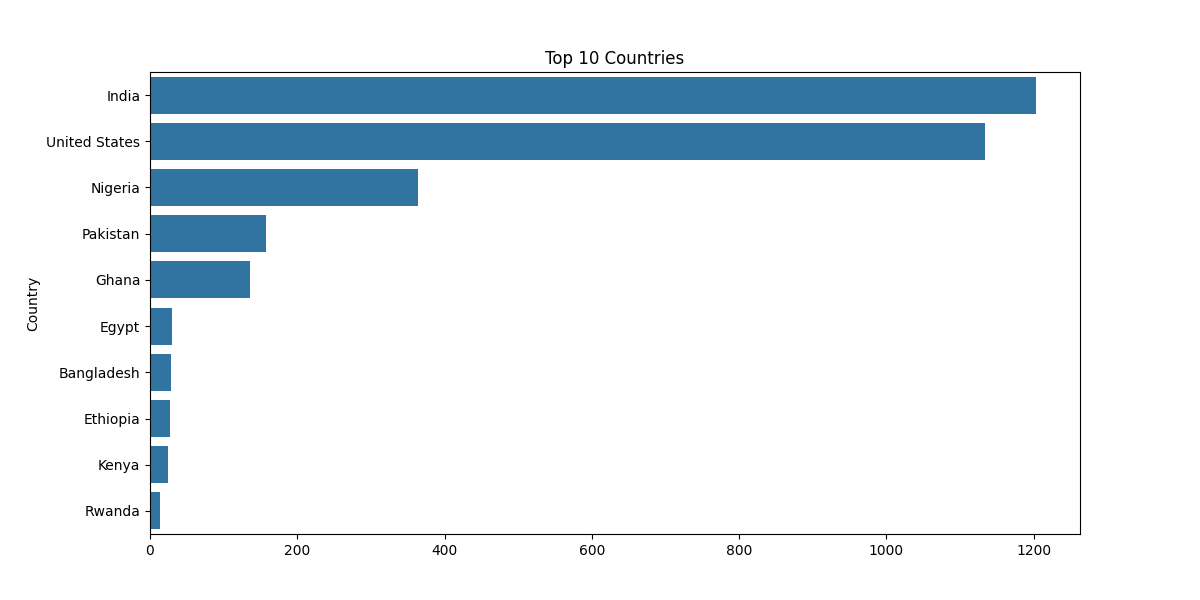
\includegraphics[width=\textwidth]{../Statistics/Figure_2.png}
    \caption{Top 10 Countries}
\end{figure}

\subsection{Monthly Signup Trend}
\begin{figure}[H]
    \centering
    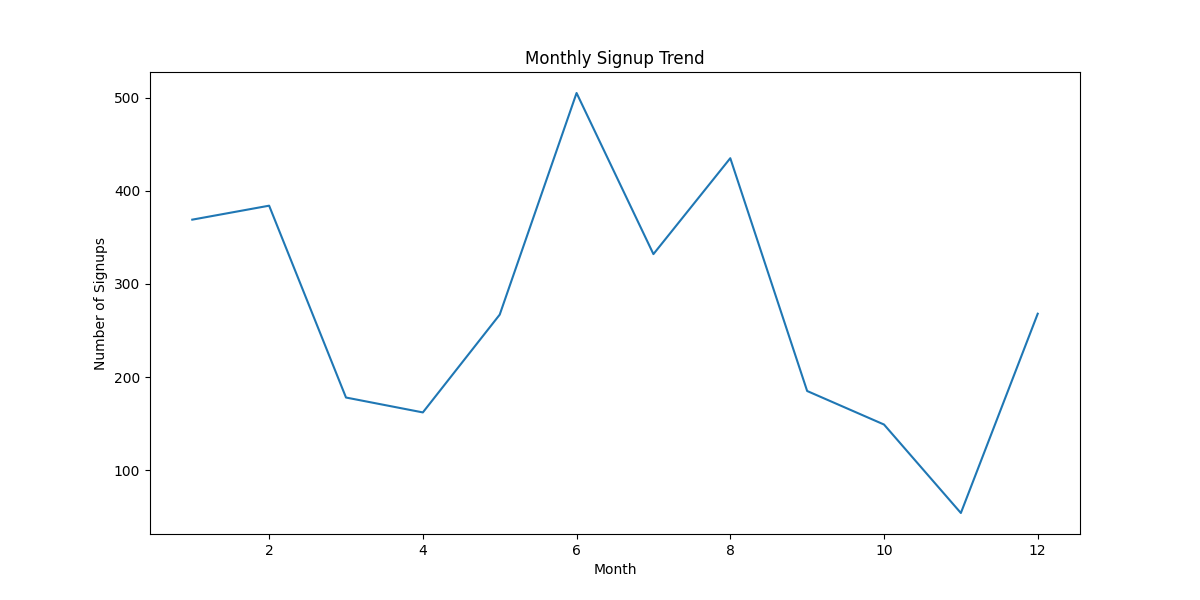
\includegraphics[width=\textwidth]{../Statistics/Figure_3.png}
    \caption{Monthly Signup Trend}
\end{figure}

\subsection{Correlation Matrix}
\begin{figure}[H]
    \centering
    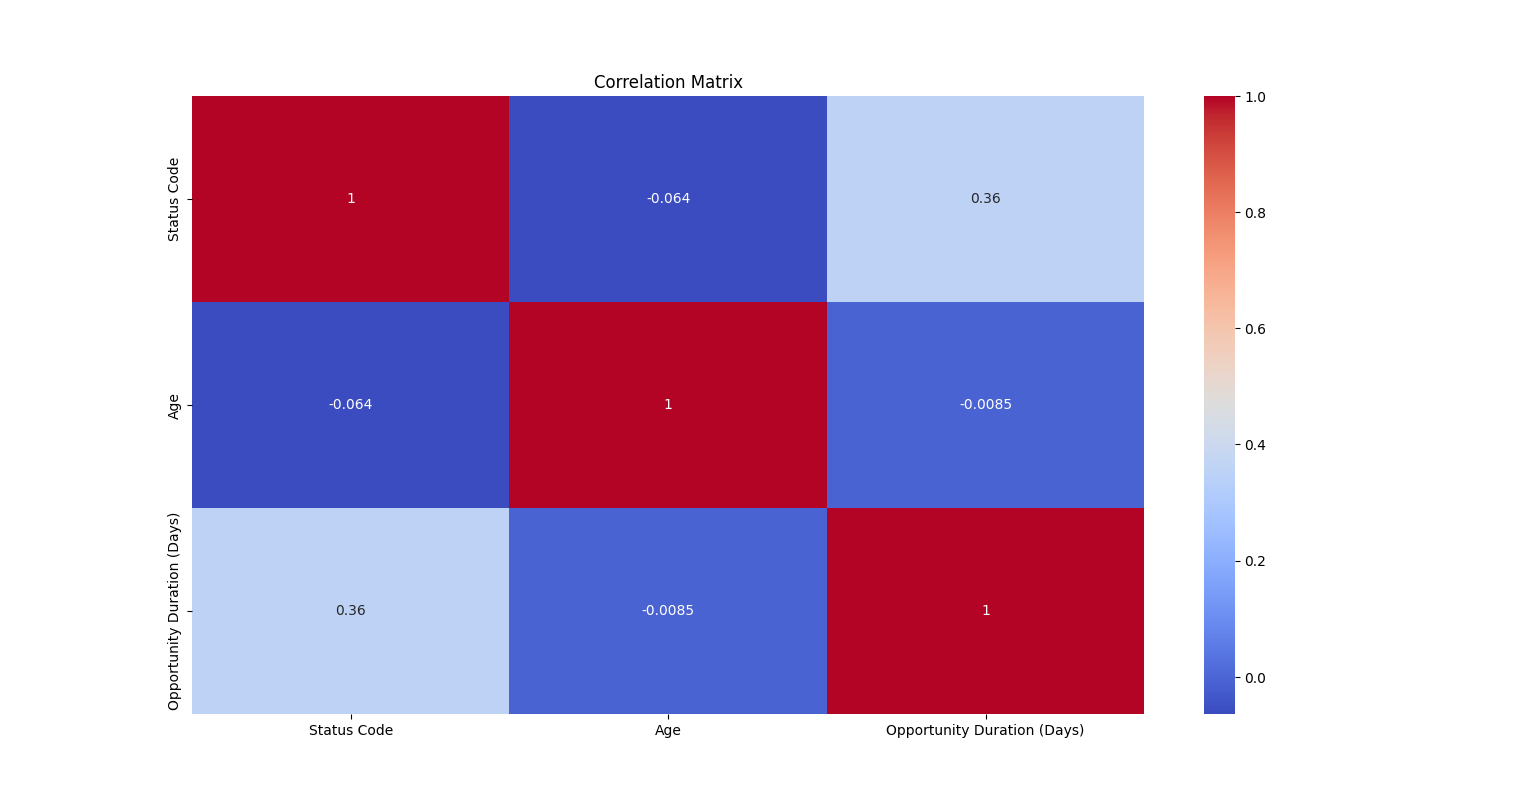
\includegraphics[width=0.8\textwidth]{../Statistics/Figure_4.png}
    \caption{Correlation Matrix}
\end{figure}

\section{Key Insights}
\begin{itemize}
    \item Top Country: India
    \item Most Common Status: Team Allocated
    \item Most Common Age: 24.0
    \item Gender Distribution: Male (55\%), Female (45\%)
    \item Average Age: 30.5 years
    \item Total Unique Participants: 1000
\end{itemize}

\section{Conclusion}
The EDA report provides a comprehensive overview of the dataset, highlighting key trends, patterns, and correlations. The insights gained from this analysis can inform decision-making processes and guide further investigations.

\section{Recommendations}
\begin{itemize}
    \item Target peak signup months with additional marketing efforts.
    \item Investigate reasons for drops in signups or completions.
    \item Provide additional resources for users with longer completion times.
    \item Develop tailored strategies for different demographic groups.
\end{itemize}

\end{document}

